\documentclass[aspectratio=169]{beamer}
\usetheme{Madrid}
\usecolortheme{crane}
%\useoutertheme{split}
\usepackage{caption,subcaption,axodraw2,color,graphicx,expl3,calc,subfig,braket,mathtools,amsmath,calc,bm,tikz}
\usetikzlibrary{tikzmark,fit,shapes.geometric}
\usepackage{rotating}
\usepackage{anyfontsize}
\usepackage[thicklines]{cancel}
\usepackage{transparent}
\usetikzlibrary{arrows}
\usepackage[absolute,overlay]{textpos}
\usepackage{layouts}
\usepackage{blindtext}


\def\compos{{\mbox{$\resizebox{.18in}{.17in}{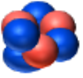
\includegraphics[clip]{./composite/composite.pdf}}$}}}
\def\rgm{  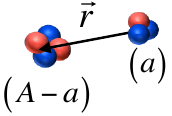
\includegraphics[scale=0.2,bb=30 30 30 30]{./composite/rgm.png}}
\def\rcurs{{\mbox{$\resizebox{.09in}{.08in}{
\includegraphics[trim= 1em 0 14em 0,clip]{./composite/ScriptR.pdf}}$}}}

\theoremstyle{remark}

\captionsetup[figure]{labelformat=empty}
\captionsetup[subfigure]{labelformat=empty}

\newtheorem*{thma}{Goal}
\newtheorem*{thmb}{Past calculations}
\newtheorem*{thmc}{New calculation}

\usepackage{mathtools}
\mathtoolsset{showonlyrefs}

\newenvironment<>{varblock}[2][.9\textwidth]{%
  \setlength{\textwidth}{#1}
  \begin{actionenv}#3%
    \def\insertblocktitle{#2}%
    \par%
    \usebeamertemplate{block begin}}
  {\par%
    \usebeamertemplate{block end}%
  \end{actionenv}}

\makeatother

\setbeamertemplate{navigation symbols}{}

 % Commands
%\newcommand{\bs}{\textbackslash}   % backslash
%\newcommand{\cmd}[1]{{\bf \color{red}#1}}   % highlights command
%\newcommand{\highlight}[1]{%
   %\colorbox{yellow}{$\displaystyle#1$}}

  %\renewcommand{\CancelColor}{\color{red}\cancel}
\newcommand\Ccancel[2][black]{\renewcommand\CancelColor{\color{#1}}\xcancel{#2}}
\usetikzlibrary{arrows,shapes,positioning}
\usetikzlibrary{decorations.markings}

\definecolor{darkred}{RGB}{128,0,0}
\definecolor{palegoldenrod}{RGB}{238,232,170}

\tikzstyle arrowstyle=[scale=1]

\tikzstyle directed=[postaction={decorate,decoration={markings,mark=at position .5 with {\arrow[arrowstyle]{stealth}}}}]
\tikzstyle reverse directed=[postaction={decorate,decoration={markings, mark=at position .5 with {\arrowreversed[arrowstyle]{stealth};}}}]

\title{\textit{Ab initio} reactions: from continuum to bound states and back}
\author{Mack C. Atkinson} 
\date{}
%\institute{Lawrence Livermore National Laboratory}
%\date{DNP Meeting 2022}

\usebackgroundtemplate{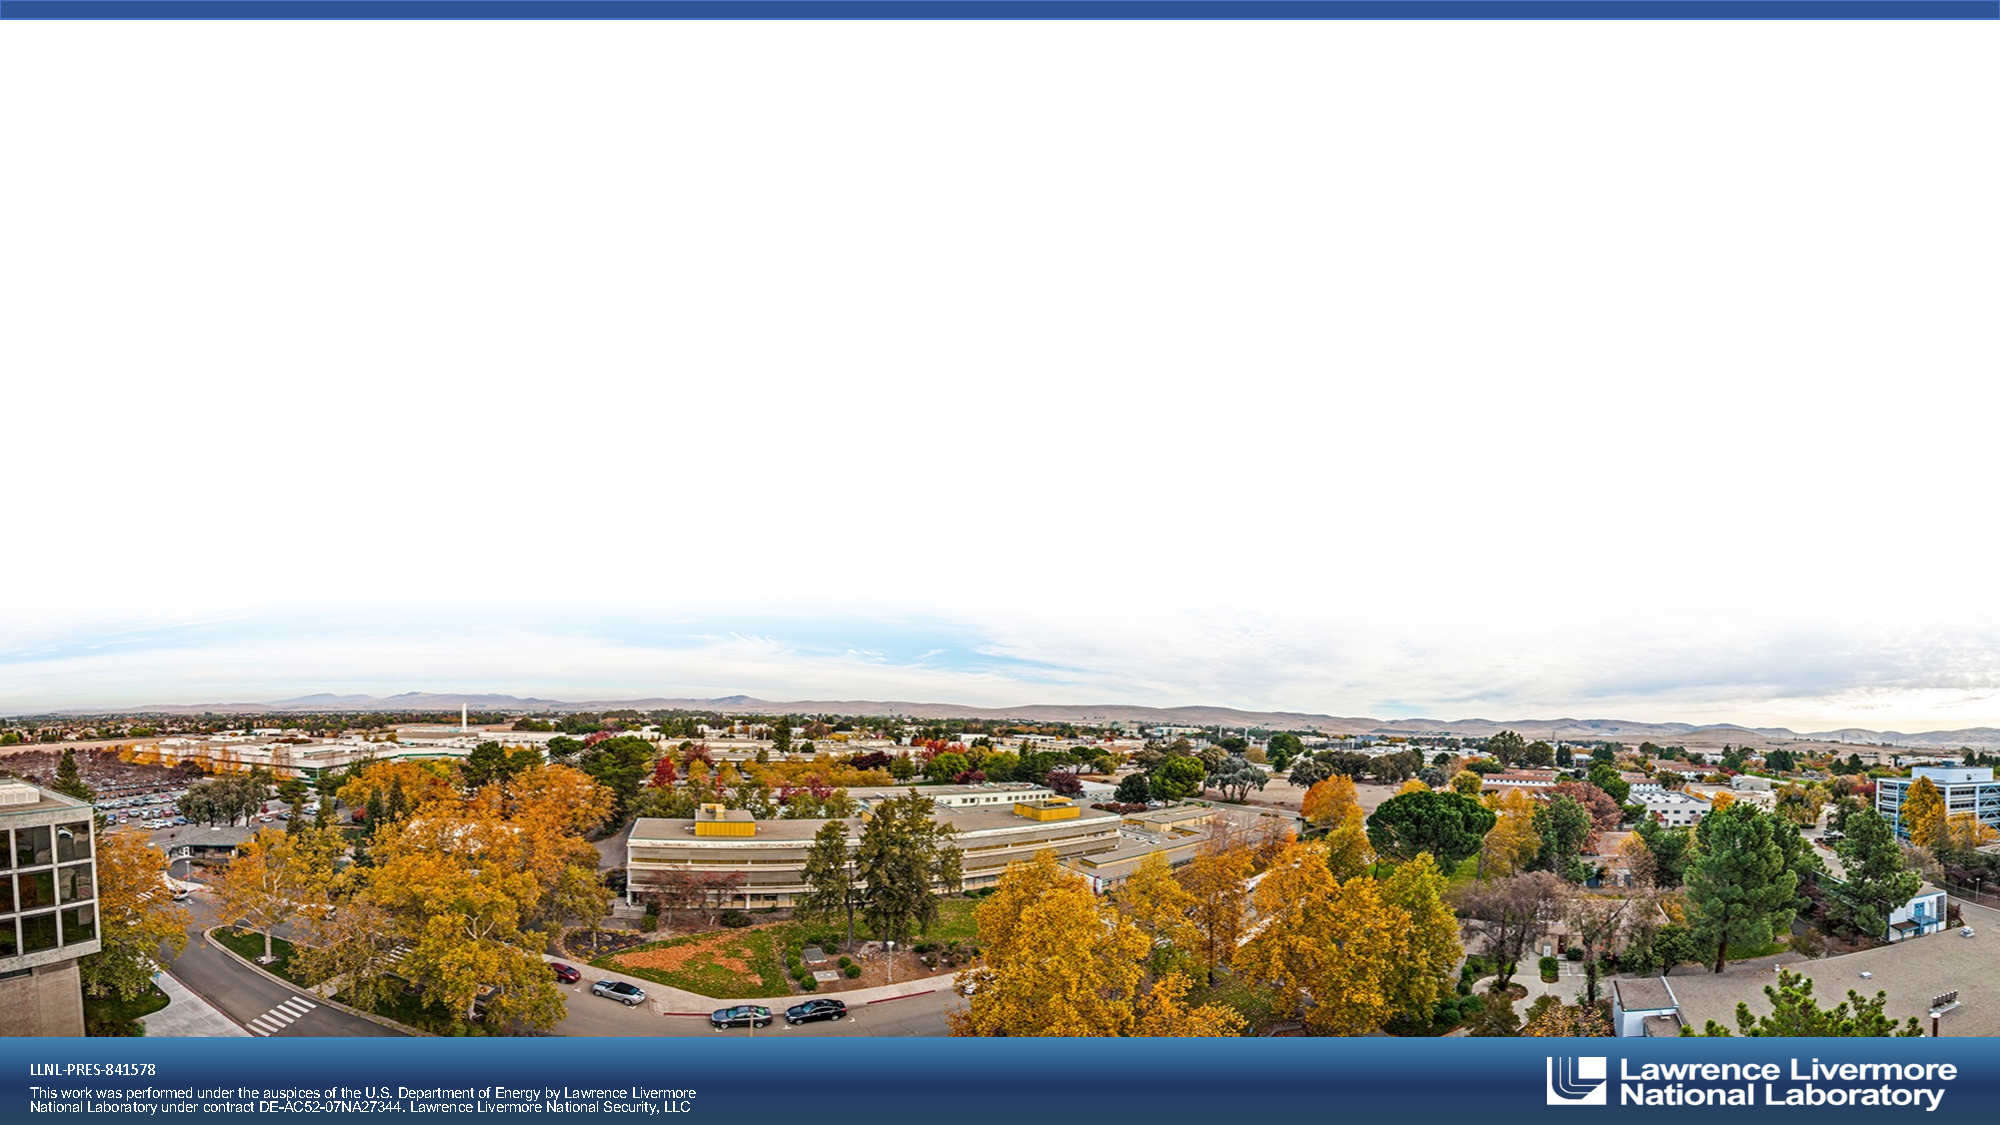
\includegraphics[width=\paperwidth, height=\paperheight]{figures/title-slide.pdf}}


\begin{document}

\hbadness=10000000

\setbeamertemplate{footline}{}

\begin{frame} 
   \titlepage

   %\begin{textblock*}{\linewidth}(8pt,219pt)
      %\begin{center}
      %\begin{varblock}[0.07\linewidth]{}
      %\end{varblock}
   %\end{center}
   %\end{textblock*}

   %\begin{textblock*}{\linewidth}(0,-10)
   %\begin{center}
      %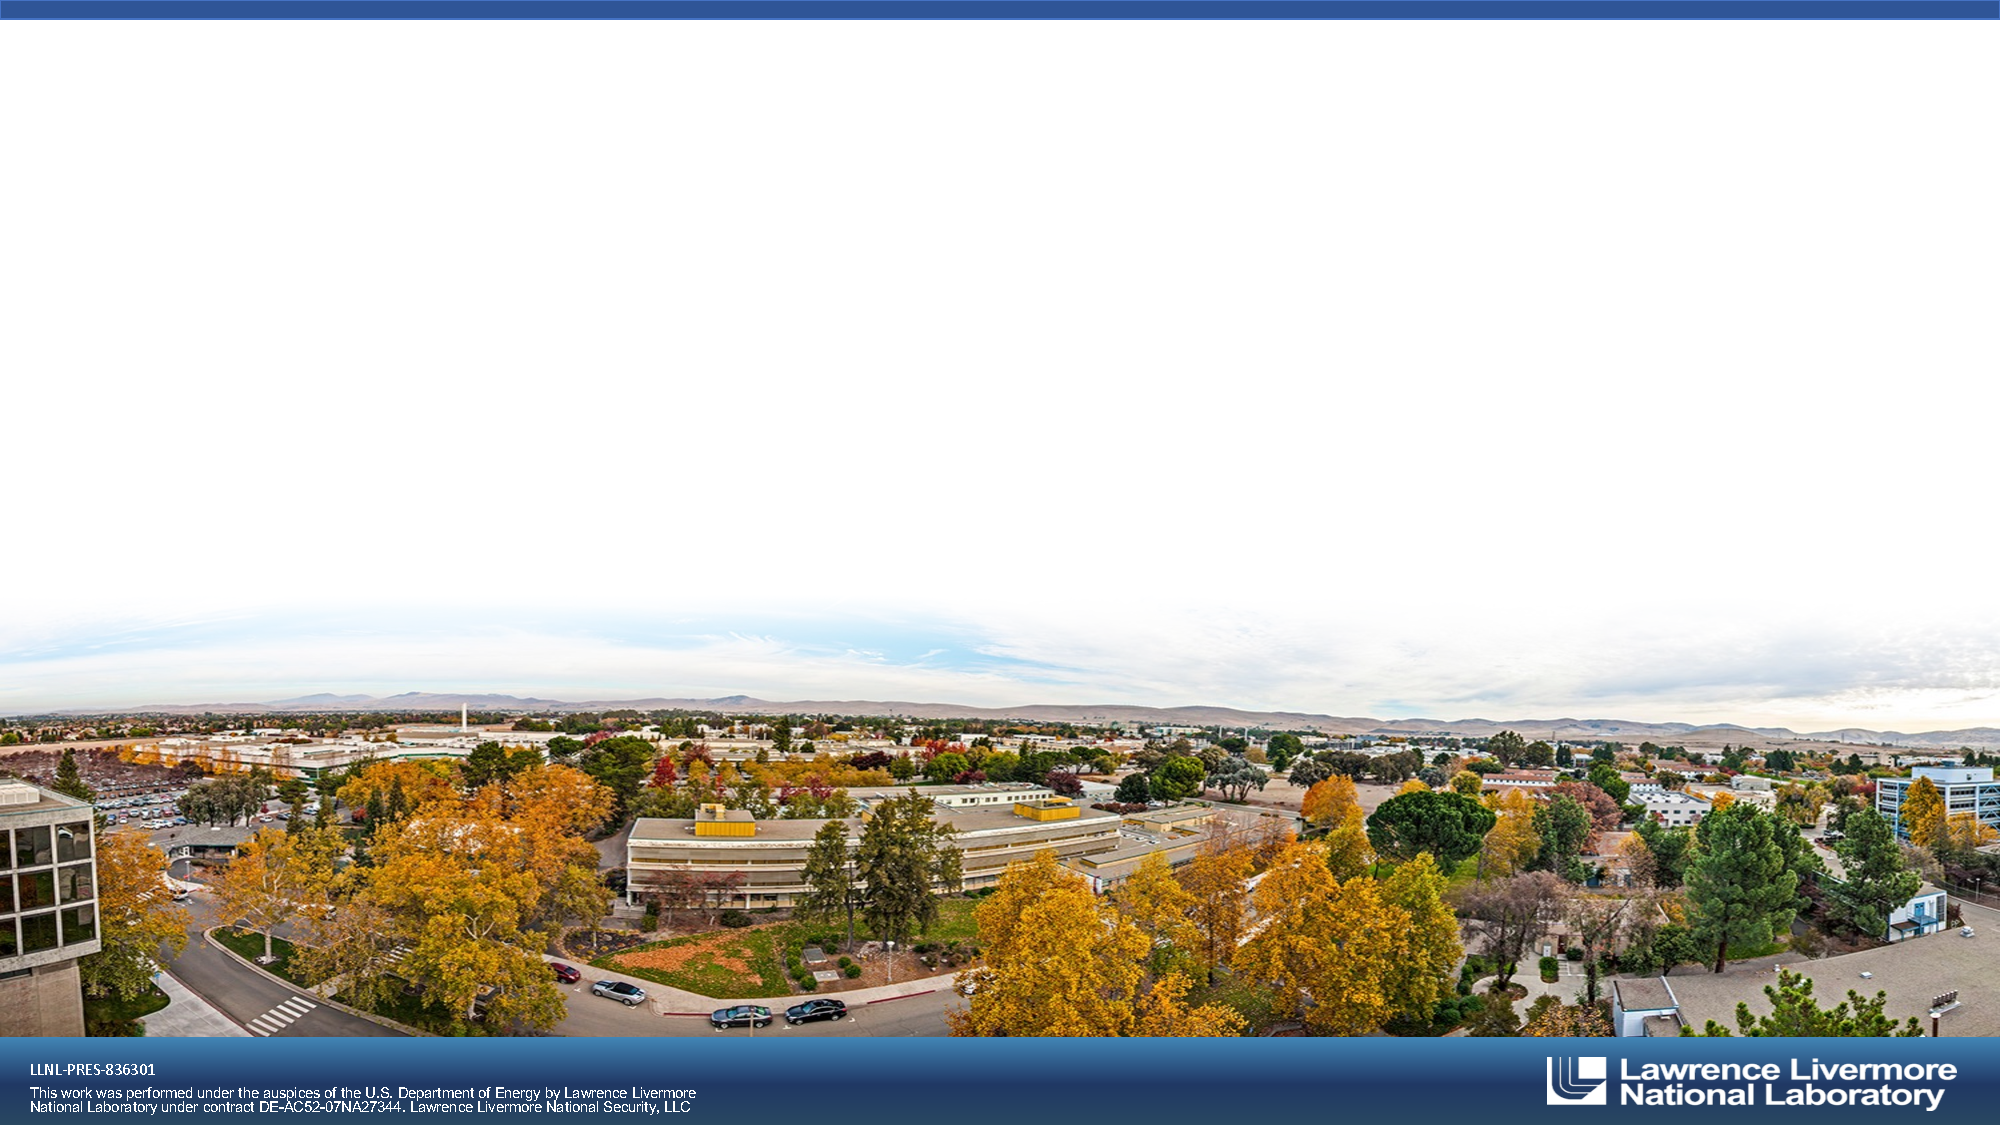
\includegraphics[scale=0.475]{figures/background.pdf}
   %\end{center}
%\end{textblock*}


   %\begin{textblock*}{100pt}(40pt,190pt)
      %\visible<2->{
      %%\includegraphics[angle=20]{figures/names.png}
         %{\small
            %\begin{rotate}{25}
               %\textcolor{blue}{Petr Navratil} 
            %\end{rotate}
         %}
      %}
   %\end{textblock*}


   %\begin{textblock*}{\linewidth}(12pt,200pt)
      %\begin{center}
      %\textcolor{blue}{arXiv 2001.07231}
   %\end{center}
   %\end{textblock*}
\end{frame}

\usebackgroundtemplate{}

\setbeamertemplate{footline}
{
  \leavevmode%
  \hbox{%
  \begin{beamercolorbox}[wd=.5\paperwidth,ht=2.25ex,dp=1ex,left]{author in head/foot}%
    \hspace{0.2cm}atkinson27@llnl.gov\hspace{0.265\paperwidth}
     \insertauthor
  \end{beamercolorbox}%
  \begin{beamercolorbox}[wd=.4\paperwidth,ht=2.25ex,dp=1ex,left]{date in head/foot}%
     %\hspace{0.2cm}\insertsection
     \hspace{0.2cm}LLNL
  \end{beamercolorbox}%
  \begin{beamercolorbox}[wd=.1\paperwidth,ht=2.25ex,dp=1ex,right]{date in head/foot}%
    \insertframenumber{}\hspace*{2ex}
  \end{beamercolorbox}}%
  \vskip0pt%
}

\begin{frame}
   \frametitle{$^3$He$(\alpha,\gamma)^7$Be important for solar-model predictions}
   \begin{textblock*}{\linewidth}(10pt,40pt)
   \begin{itemize}
         \visible<4->{
      \item Reaction rates too low at solar energies in the lab
      }
      \visible<5->{
      \item Current evaluations depend on both theory and experiment 
      }
      \visible<6->{
      \item Ideally, theory will accurately predict $S_{34}(0)$
      }
   \end{itemize}
\end{textblock*}

   \begin{textblock*}{0.5\linewidth}(0.55\linewidth,190pt)
      \visible<2->{
   \begin{equation}
      \sigma(E) = \frac{S_{34}(E)}{E}\textrm{exp}\left\{-\frac{2\pi Z_1Z_2e^2}{\hbar\sqrt{2E/m}}\right\}
   \end{equation}
}
\end{textblock*}

   \begin{textblock*}{0.5\linewidth}(0.6\linewidth,25pt)
      \visible<1->{
   \begin{center}
      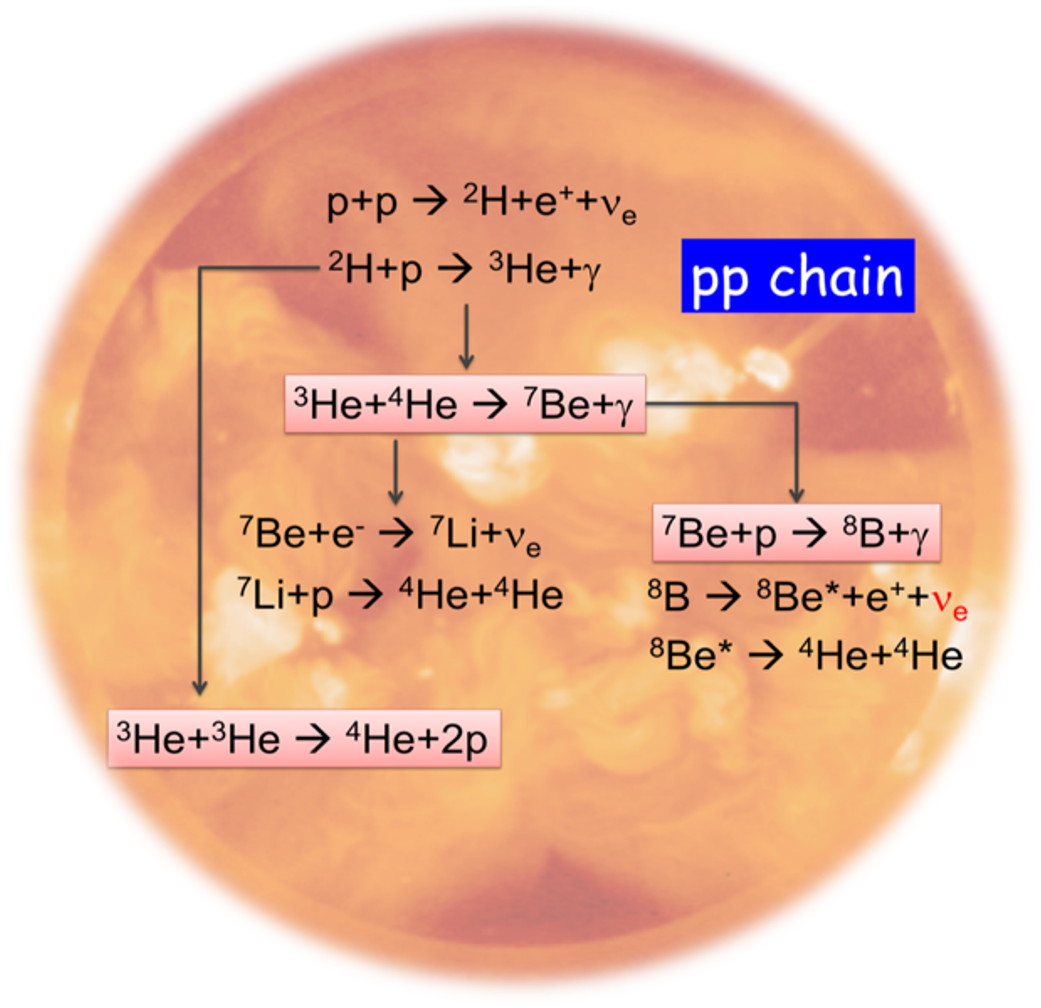
\includegraphics[scale=0.4]{figures/solar-fusion.png}
   \end{center}
}
\end{textblock*}

   \begin{textblock*}{0.5\linewidth}(10pt,100pt)
      \visible<3->{
   \begin{center}
      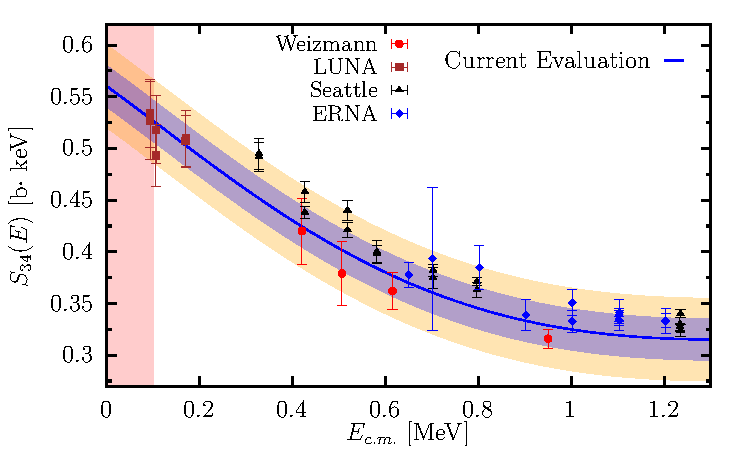
\includegraphics[scale=0.6]{figures/capture-zoomed_model}
   \end{center}
}
\end{textblock*}

   \begin{textblock*}{200pt}(-10pt,241pt)
      \visible<3->{
         \fontsize{6}{5.2}\selectfont \quad \quad Adelberger \textit{et al}., Rev Mod Phys \textbf{83} 195 (2011)
      }
   \end{textblock*}

\end{frame}

\begin{frame}
   %\frametitle{Outline}
   \frametitle{\textbf{Goal}: Improve the theoretical prediction of $S_{34}(E)$}
   %\begin{thma}
      %Reduce the theoretical uncertainty in the determination of S_{34}(0)
   %\end{thma}

   \begin{textblock*}{\linewidth}(100pt,20pt)
      \begin{center}
         \visible<1->{
      \begin{varblock}[0.58\linewidth]{}
         Current evaluation:
            \begin{equation}
               S_{34}(0) = 0.56 \pm 0.02\textrm{(expt.)}\pm \mathbf{0.02}\textrm{\textbf{(theor.)}}
            \end{equation}
      \end{varblock}
   }
   \end{center}
   \end{textblock*}

   %\begin{equation}
      %S_{34}(0) = 0.56 \pm 0.02\textrm{(expt.)}\pm \mathbf{0.02}\textrm{\textbf{(theor)}}
   %\end{equation}

   \begin{textblock*}{\linewidth}(10pt,90pt)
   \begin{itemize}
         \visible<2->{
      \item \textbf{How?}: Perform an \textit{ab initio} calculation of the $^3$He$(\alpha,\gamma)^7$Be reaction 
      }
         \begin{itemize}
               \visible<3->{
      \item Previously only possible using NN forces
      }
   \end{itemize}
   \end{itemize}
\end{textblock*}

   \begin{textblock*}{0.7\linewidth}(10pt,115pt)
      \begin{center}
         \visible<4->{
      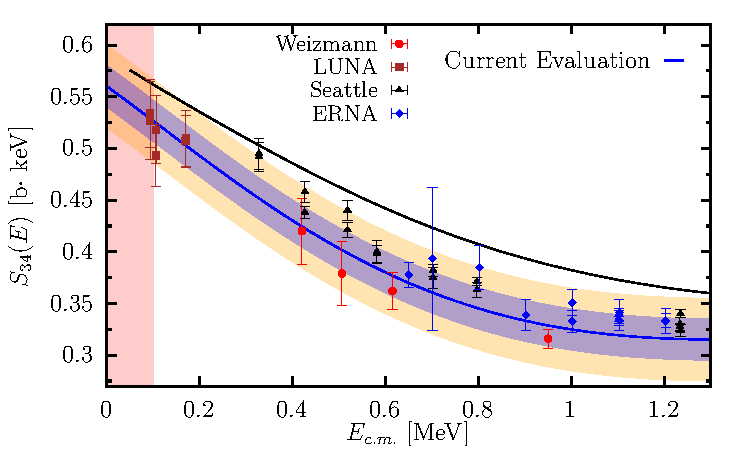
\includegraphics[scale=0.45]{figures/capture-zoomed}
   }
   \end{center}
\end{textblock*}

   \begin{textblock*}{0.7\linewidth}(165pt,152pt)
      \visible<4->{
      \begin{tikzpicture}
         \draw [thick, -stealth] (0,0) -- (-0.5,-0.5);
      \end{tikzpicture}
   }
   \end{textblock*}

   \begin{textblock*}{0.2\linewidth}(181pt,150pt)
      \visible<4->{
         {\tiny NN only}
   }
   \end{textblock*}

   \begin{textblock*}{0.4\linewidth}(0.65\linewidth,110pt)
      \begin{center}
         \visible<5->{
      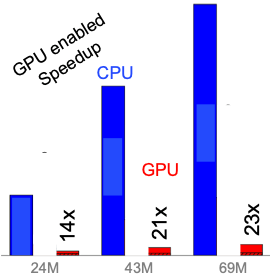
\includegraphics[scale=0.4]{figures/boost.png}
   }
   \end{center}
\end{textblock*}

   \begin{textblock*}{\linewidth}(10pt,230pt)
   \begin{itemize}
      %\item I present the first \textit{ab initio} calculation of $^3$He$(\alpha,\gamma)^7$Be including NN forces
         \visible<6->{
      \item GPU speedup $\implies$ NNN forces are now included
      }
   \end{itemize}
\end{textblock*}

\end{frame}

\begin{frame}
   \frametitle{The \textit{ab initio} method: from NCSM to NCSMC}

   \begin{textblock*}{0.3\linewidth}(10pt,40pt)
      \visible<3->{
         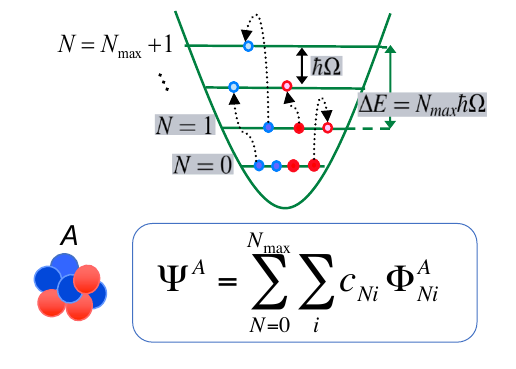
\includegraphics[scale=0.3]{figures/ncsm.png}
      }
   \end{textblock*}

   \begin{textblock*}{0.3\linewidth}(10pt,40pt)

      \visible<5->{
      \begin{tikzpicture}
         \node[rectangle,dashed,very thick,draw,minimum width=4.1cm,minimum height=6cm] (r) at (0,0) {};
      \end{tikzpicture}
   }

   \end{textblock*}

   \begin{textblock*}{0.3\linewidth}(5pt,115pt)
      \visible<4->{
         \begin{equation}
            \hat{H} = \hat{T}+\hat{V}_{NN}+\hat{V}_{NNN}
         \end{equation}
         \begin{equation}
            \hat{H}\ket{\Psi^A} = E\ket{\Psi^A}
         \end{equation}
      }
   \end{textblock*}

   %\begin{textblock*}{0.3\linewidth}(10pt,130pt)
      %\visible<2->{
         %\begin{equation}
            %\hat{H}\ket{\Psi^A} = E\ket{\Psi^A}
         %\end{equation}
      %}
   %\end{textblock*}

   \begin{textblock*}{0.3\linewidth}(52pt,175pt)
      \visible<5->{
         %{\Large NCSM}
         \begin{varblock}[0.3\linewidth]{}
            \Large NCSM
         \end{varblock}
      }
   \end{textblock*}

   \begin{textblock*}{0.2\linewidth}(0.65\linewidth,25pt)
      \visible<10->{
         %{\Large NCSM}
         \begin{varblock}[0.55\linewidth]{}
            \Large NCSMC
         \end{varblock}
      }
   \end{textblock*}

   \begin{textblock*}{0.5\linewidth}(0.45\linewidth,60pt)
      \visible<6->{
         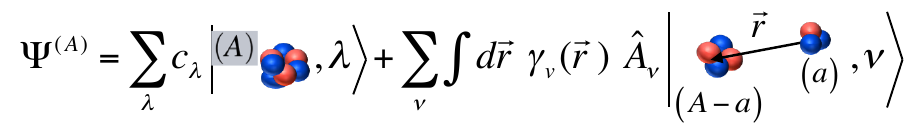
\includegraphics[scale=0.3]{figures/ncsmc_wavefunction.png}
      }
   \end{textblock*}

   %\begin{textblock*}{0.5\linewidth}(0.45\linewidth,30pt)
      %\visible<7->{
      %\begin{tikzpicture}
         %\node[rectangle,dashed,very thick,draw,minimum width=8.1cm,minimum height=2cm] (r) at (0,0) {};
      %\end{tikzpicture}
   %}
   %\end{textblock*}

   \begin{textblock*}{0.9\linewidth}(5pt,30pt)
      \visible<10->{
      \begin{tikzpicture}
         \node[rectangle,thick,draw,minimum width=1.1\linewidth,minimum height=6.7cm] (r) at (0,0) {};
      \end{tikzpicture}
   }
   \end{textblock*}

   \begin{textblock*}{0.05\linewidth}(0.6\linewidth,90pt)
      \visible<7->{
      \begin{tikzpicture}
         \draw [thick, stealth-] (0,0) -- (0,-0.5);
      \end{tikzpicture}
   }
   \end{textblock*}

   \begin{textblock*}{0.3\linewidth}(0.45\linewidth,105pt)
      \visible<7->{
      {\Large
      \begin{equation}
         \ket{{}^{7}\textrm{Be}}
      \end{equation}
   }
   }
   \end{textblock*}

   \begin{textblock*}{0.05\linewidth}(0.85\linewidth,90pt)
      \visible<8->{
      \begin{tikzpicture}
         \draw [thick, stealth-] (0,0) -- (0,-0.5);
      \end{tikzpicture}
   }
   \end{textblock*}


   \begin{textblock*}{0.3\linewidth}(0.7\linewidth,105pt)
      \visible<8->{
      {\Large
         \begin{equation}
         \ket{\alpha} \otimes \ket{^3\textrm{He}}
      \end{equation}
      }
      }
   \end{textblock*}

   \begin{textblock*}{0.5\linewidth}(0.3\linewidth,120pt)
      \visible<9->{
      \begin{tikzpicture}
         \draw [dashed, thick, stealth-] (0.95,-0.20) [out=210, in=-50] to (-7.3,0);
      \end{tikzpicture}
   }
   \end{textblock*}

   \begin{textblock*}{0.5\linewidth}(0.3\linewidth,120pt)
      \visible<9->{
      \begin{tikzpicture}
         \draw [dashed, thick, stealth-] (-3,-0.20) [out=210, in=-50] to (-7.3,0.2);
      \end{tikzpicture}
   }
   \end{textblock*}


   \begin{textblock*}{0.55\linewidth}(0.35\linewidth,180pt)
      \begin{varblock}[\linewidth]{}
      \Large
      \vspace{-3mm}
      \begin{equation}
         \Braket{\Psi_{bs}\left(^7\textrm{Be}\right)|\hat{\mathcal{M}}_{\mathrm{EM}}|\Psi_{sc}\left(^3\textrm{He}+\alpha\right)}$
     \end{equation}
     \vspace{-2cm}
        %$\Braket{\Psi_{bs}\left(^7\textrm{Be}\right)|(\bm{E}+\bm{M})|\Psi_{sc}\left(^3\textrm{He}+\alpha\right)}$
   \end{varblock}
   \end{textblock*}

   \begin{textblock*}{0.1\linewidth}(0.91\linewidth,180pt)
      \visible<2-10>{
      
\includegraphics[scale=0.07]{figures/question-mark.png}
   }
   \end{textblock*}

   \begin{textblock*}{0.1\linewidth}(0.91\linewidth,180pt)
      \visible<11->{
      
\includegraphics[scale=0.092]{figures/check-mark.png}
   }
   \end{textblock*}

   %\begin{textblock*}{0.3\linewidth}(0.35\linewidth,180pt)
      %\visible<8->{
         %\begin{equation}
            %\Braket{\Psi^{(A)}_\textrm{\tiny NCSMC}|\hat{H}|\Psi^{(A)}_\textrm{\tiny NCSMC}} \implies
         %\end{equation}
      %}
   %\end{textblock*}

   %\begin{textblock*}{0.3\linewidth}(0.7\linewidth,160pt)
      %\visible<9->{
         %\begin{equation}
            %\Braket{^{^{(A)}}\compos|\hat{H}|^{^{(A)}}\compos}
         %\end{equation}
      %}
      %\begin{equation}
         %\Ket{\rgm} = \Ket{\rcurs}
      %\end{equation}
   %\end{textblock*}

\end{frame}

\begin{frame}
   \frametitle{NCSMC Calculation of $^{3}$He$+^{4}$He shows reasonable agreement with data}

   \begin{textblock*}{\linewidth}(20pt,30pt)
      \visible<2->{
      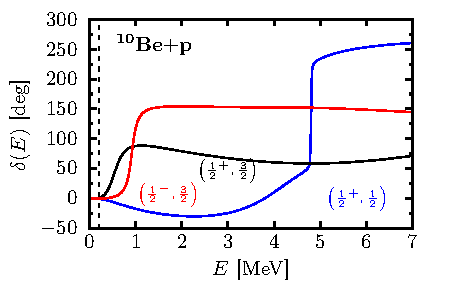
\includegraphics[scale=0.8]{figures/phase.pdf}
   }
   \end{textblock*}

   \begin{textblock*}{\linewidth}(20pt,130pt)
      \visible<2->{
      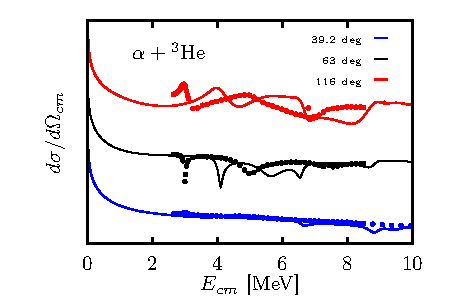
\includegraphics[scale=0.8]{figures/xsec-angle.pdf}
   }
   \end{textblock*}

   \begin{textblock*}{0.5\linewidth}(0.35\linewidth,130pt)
      \visible<3->{
         \begin{center}
            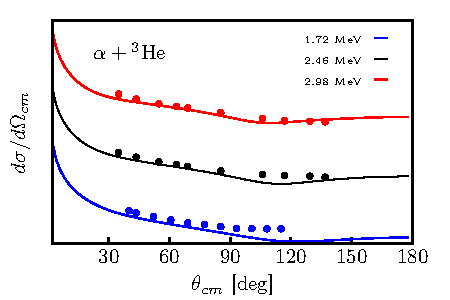
\includegraphics[scale=0.7]{figures/xsec.pdf}
         \end{center}
      }
   \end{textblock*}

   \begin{textblock*}{0.5\linewidth}(0.65\linewidth,30pt)
      \visible<1->{
         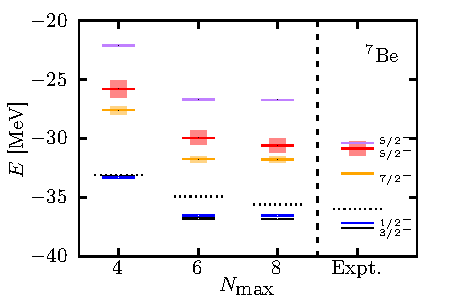
\includegraphics[scale=0.8]{figures/ncsm-nmax}
      }
   \end{textblock*}

   \begin{textblock*}{\linewidth}(0.88\linewidth,150pt)
      \begin{varblock}[0.15\linewidth]{}
         {\fontsize{8pt}{7.2}\selectfont NN-N3LO+3Nlnl} \\
         {\fontsize{8pt}{7.2}\selectfont$\hbar\Omega=20$ MeV} \\
         {\fontsize{8pt}{7.2}\selectfont$\lambda_{\mathrm{SRG}} = 2.0$ fm$^{-1}$}
      \end{varblock}
   \end{textblock*}

   \begin{textblock*}{200pt}(315pt,240pt)
      \visible<1->{
         \fontsize{6}{5.2}\selectfont \quad \quad P. Navratil, Few Body Systems {\bf 41}, 117 (2007)
      }
   \end{textblock*}

   \begin{textblock*}{200pt}(292pt,234pt)
      \visible<1->{
         \fontsize{6}{5.2}\selectfont \quad \quad D.R. Entem and R. Machleidt, PRC {\bf 68}, 041001 (2003)
      }
   \end{textblock*}

\end{frame}

\begin{frame}
   \frametitle{Results are promising but convergence needs to be explored}
   \begin{textblock*}{\linewidth}(10pt,30pt)
   \end{textblock*}

   \begin{textblock*}{\linewidth}(0.88\linewidth,30pt)
      \begin{varblock}[0.15\linewidth]{}
         {\fontsize{8pt}{7.2}\selectfont NN-N3LO+3Nlnl} \\
         {\fontsize{8pt}{7.2}\selectfont$\hbar\Omega=20$ MeV} \\
         {\fontsize{8pt}{7.2}\selectfont$\lambda_{\mathrm{SRG}} = 2.0$ fm$^{-1}$}
      \end{varblock}
   \end{textblock*}

   \begin{textblock*}{0.3\linewidth}(10pt,20pt)
      \begin{center}
         \visible<2->{
            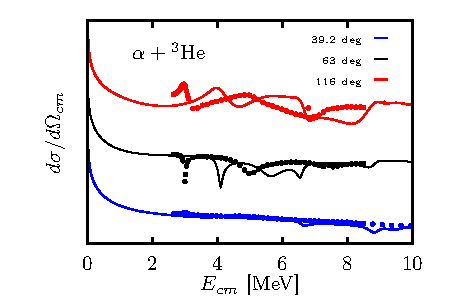
\includegraphics[scale=0.65]{figures/xsec-angle.pdf}
         }
      \end{center}
   \end{textblock*}

   \begin{textblock*}{0.2\linewidth}(80pt,130pt)
      \visible<3->{
         {\Huge $+$}
      }
   \end{textblock*}

   \begin{textblock*}{0.3\linewidth}(10pt,140pt)
      \begin{center}
         \visible<4->{
            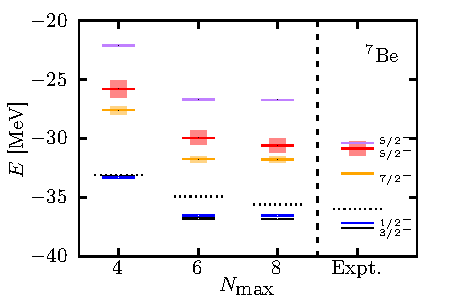
\includegraphics[scale=0.65]{figures/ncsm-nmax.pdf}
         }
      \end{center}
   \end{textblock*}

   \begin{textblock*}{0.2\linewidth}(130pt,135pt)
      \visible<5->{
         {\Huge $\implies$}
      }
   \end{textblock*}

   \begin{textblock*}{0.7\linewidth}(200pt,30pt)
      \begin{center}
         \visible<1->{
            \begin{varblock}[0.3\linewidth]{}
               $^3\textrm{He}+\alpha \rightarrow {}^7\textrm{Be} + \gamma$
            %$^3$He$+\alpha \rightarrow ^7$Be$ + \gamma$
            \end{varblock}
         }
      \end{center}
   \end{textblock*}

   \begin{textblock*}{0.7\linewidth}(170pt,80pt)
      \begin{center}
         \visible<6>{
            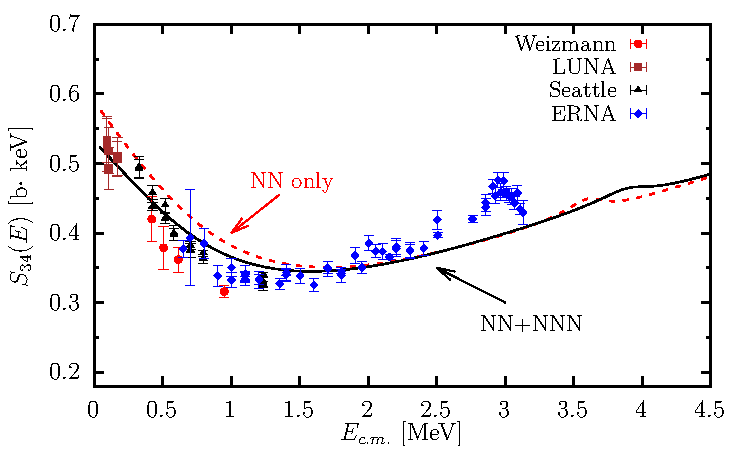
\includegraphics[scale=0.7]{figures/capture.pdf}
         }
      \end{center}
   \end{textblock*}

   \begin{textblock*}{0.7\linewidth}(170pt,80pt)
      \begin{center}
         \visible<7->{
            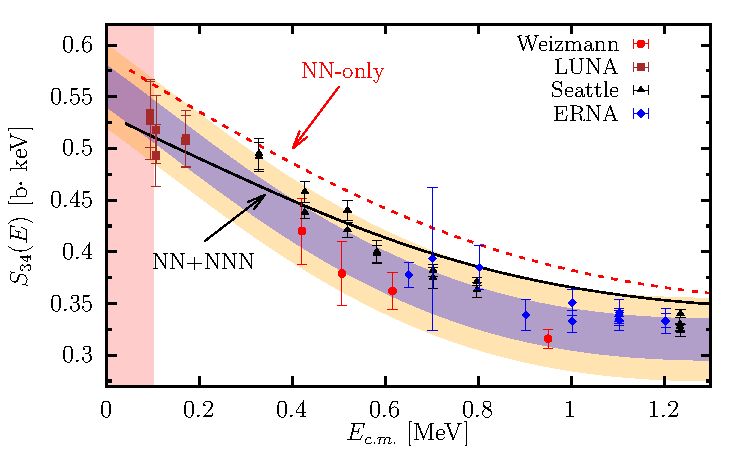
\includegraphics[scale=0.7]{figures/capture-zoomed_comp.pdf}
         }
      \end{center}
   \end{textblock*}

   %\begin{textblock*}{\linewidth}(0pt,80pt)
      %\begin{center}
         %\visible<2->{
            %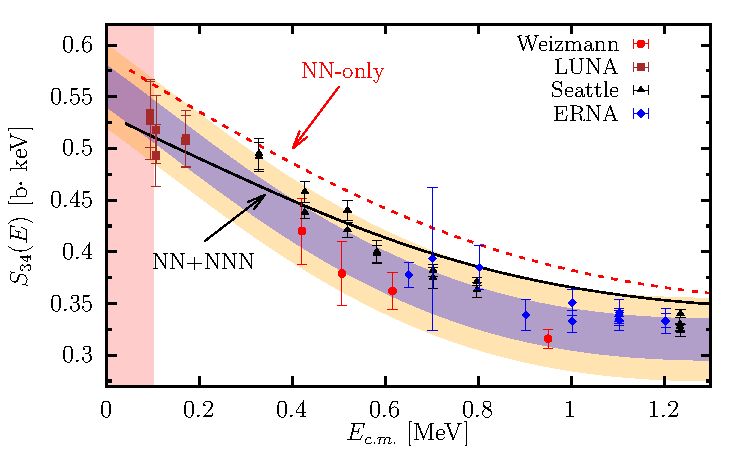
\includegraphics[scale=0.6]{figures/capture-zoomed_comp.pdf}
         %}
      %\end{center}
   %\end{textblock*}

   \begin{textblock*}{8.1cm}(240pt,210pt)
      \visible<6->{
         \begin{rotate}{10}
            {\transparent{0.2} \fontsize{15}{20}\selectfont \textcolor{red}{Preliminary}}
         \end{rotate}
      }
   \end{textblock*}


\end{frame}

%\begin{frame}
   %\frametitle{Results are promising but convergence needs to be explored}
   %\begin{textblock*}{\linewidth}(10pt,30pt)
   %\end{textblock*}

   %\begin{textblock*}{\linewidth}(0pt,80pt)
      %\begin{center}
         %\visible<1>{
            %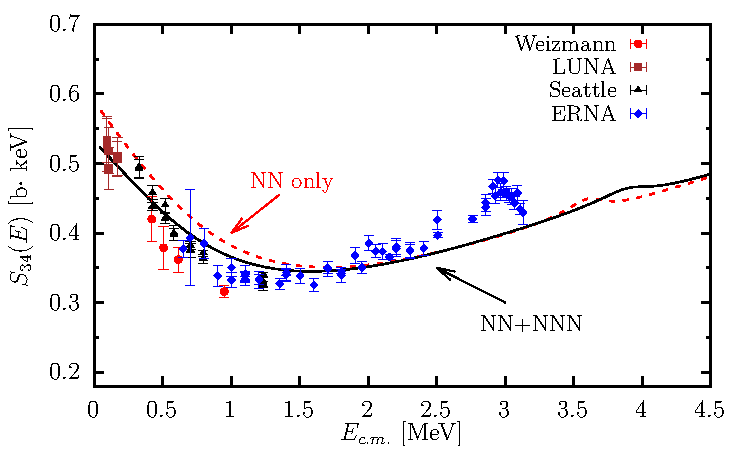
\includegraphics[scale=0.7]{figures/capture.pdf}
         %}
      %\end{center}
   %\end{textblock*}

   %\begin{textblock*}{\linewidth}(0pt,80pt)
      %\begin{center}
         %\visible<2->{
            %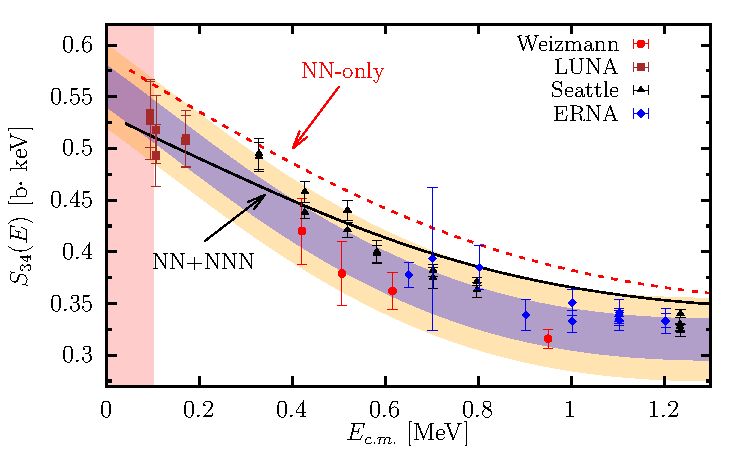
\includegraphics[scale=0.7]{figures/capture-zoomed_comp.pdf}
         %}
      %\end{center}
   %\end{textblock*}

   %\begin{textblock*}{8.1cm}(280pt,150pt)
      %\begin{rotate}{20}
         %{\transparent{0.2} \fontsize{30}{40}\selectfont \textcolor{red}{Preliminary}}
      %\end{rotate}
   %\end{textblock*}

%\end{frame}

%\begin{frame}
   %\frametitle{Moving Forward}
   %\begin{itemize}
      %\item Vary which chiral NN and NNN interactions are used to provide a theoretical uncertainty
   %\end{itemize}
%\end{frame}

\begin{frame}
   \frametitle{Thanks}

   \begin{textblock*}{0.45\linewidth}(10pt,50pt)
      \begin{varblock}[\linewidth]{}
         \begin{center}
            \begin{figure}
               \begin{subfigure}[b]{3cm}
                  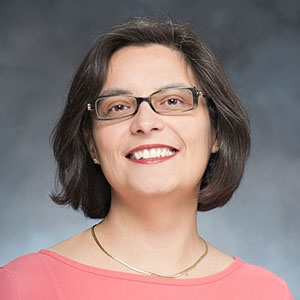
\includegraphics[width=3cm]{figures/sofia.png}
                  \caption{Sofia Quaglioni}
               \end{subfigure}
               \hfill
               \begin{subfigure}[b]{3cm}
                  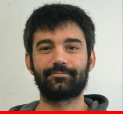
\includegraphics[width=3cm]{figures/kostas.png}
                  \caption{Kostas Kravvaris}
               \end{subfigure}
               \caption{(LLNL)}
            \end{figure}
         \end{center}
      \end{varblock}
   \end{textblock*}

   \begin{textblock*}{0.24\linewidth}(0.505\linewidth,50pt)
      \begin{varblock}[\linewidth]{}
         %\begin{center}
            %Guillame Hupin (IN2P3)
         %\end{center}
         %\vspace{-0.3cm}
         \begin{center}
      %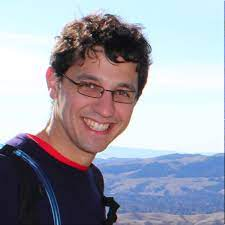
\includegraphics[scale=0.4]{figures/guillame.jpeg}
            \begin{figure}
               \begin{subfigure}{3cm}
            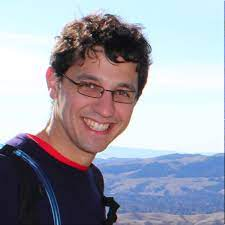
\includegraphics[width=3cm]{figures/guillame.jpeg}
            \caption{Guillame Hupin}
         \end{subfigure}
            \caption{(IN2P3)}
         \end{figure}
         \end{center}
      \end{varblock}
   \end{textblock*}

   \begin{textblock*}{0.24\linewidth}(0.78\linewidth,50pt)
      \begin{varblock}[\linewidth]{}
         \begin{center}
            \begin{figure}
               \begin{subfigure}{3cm}
            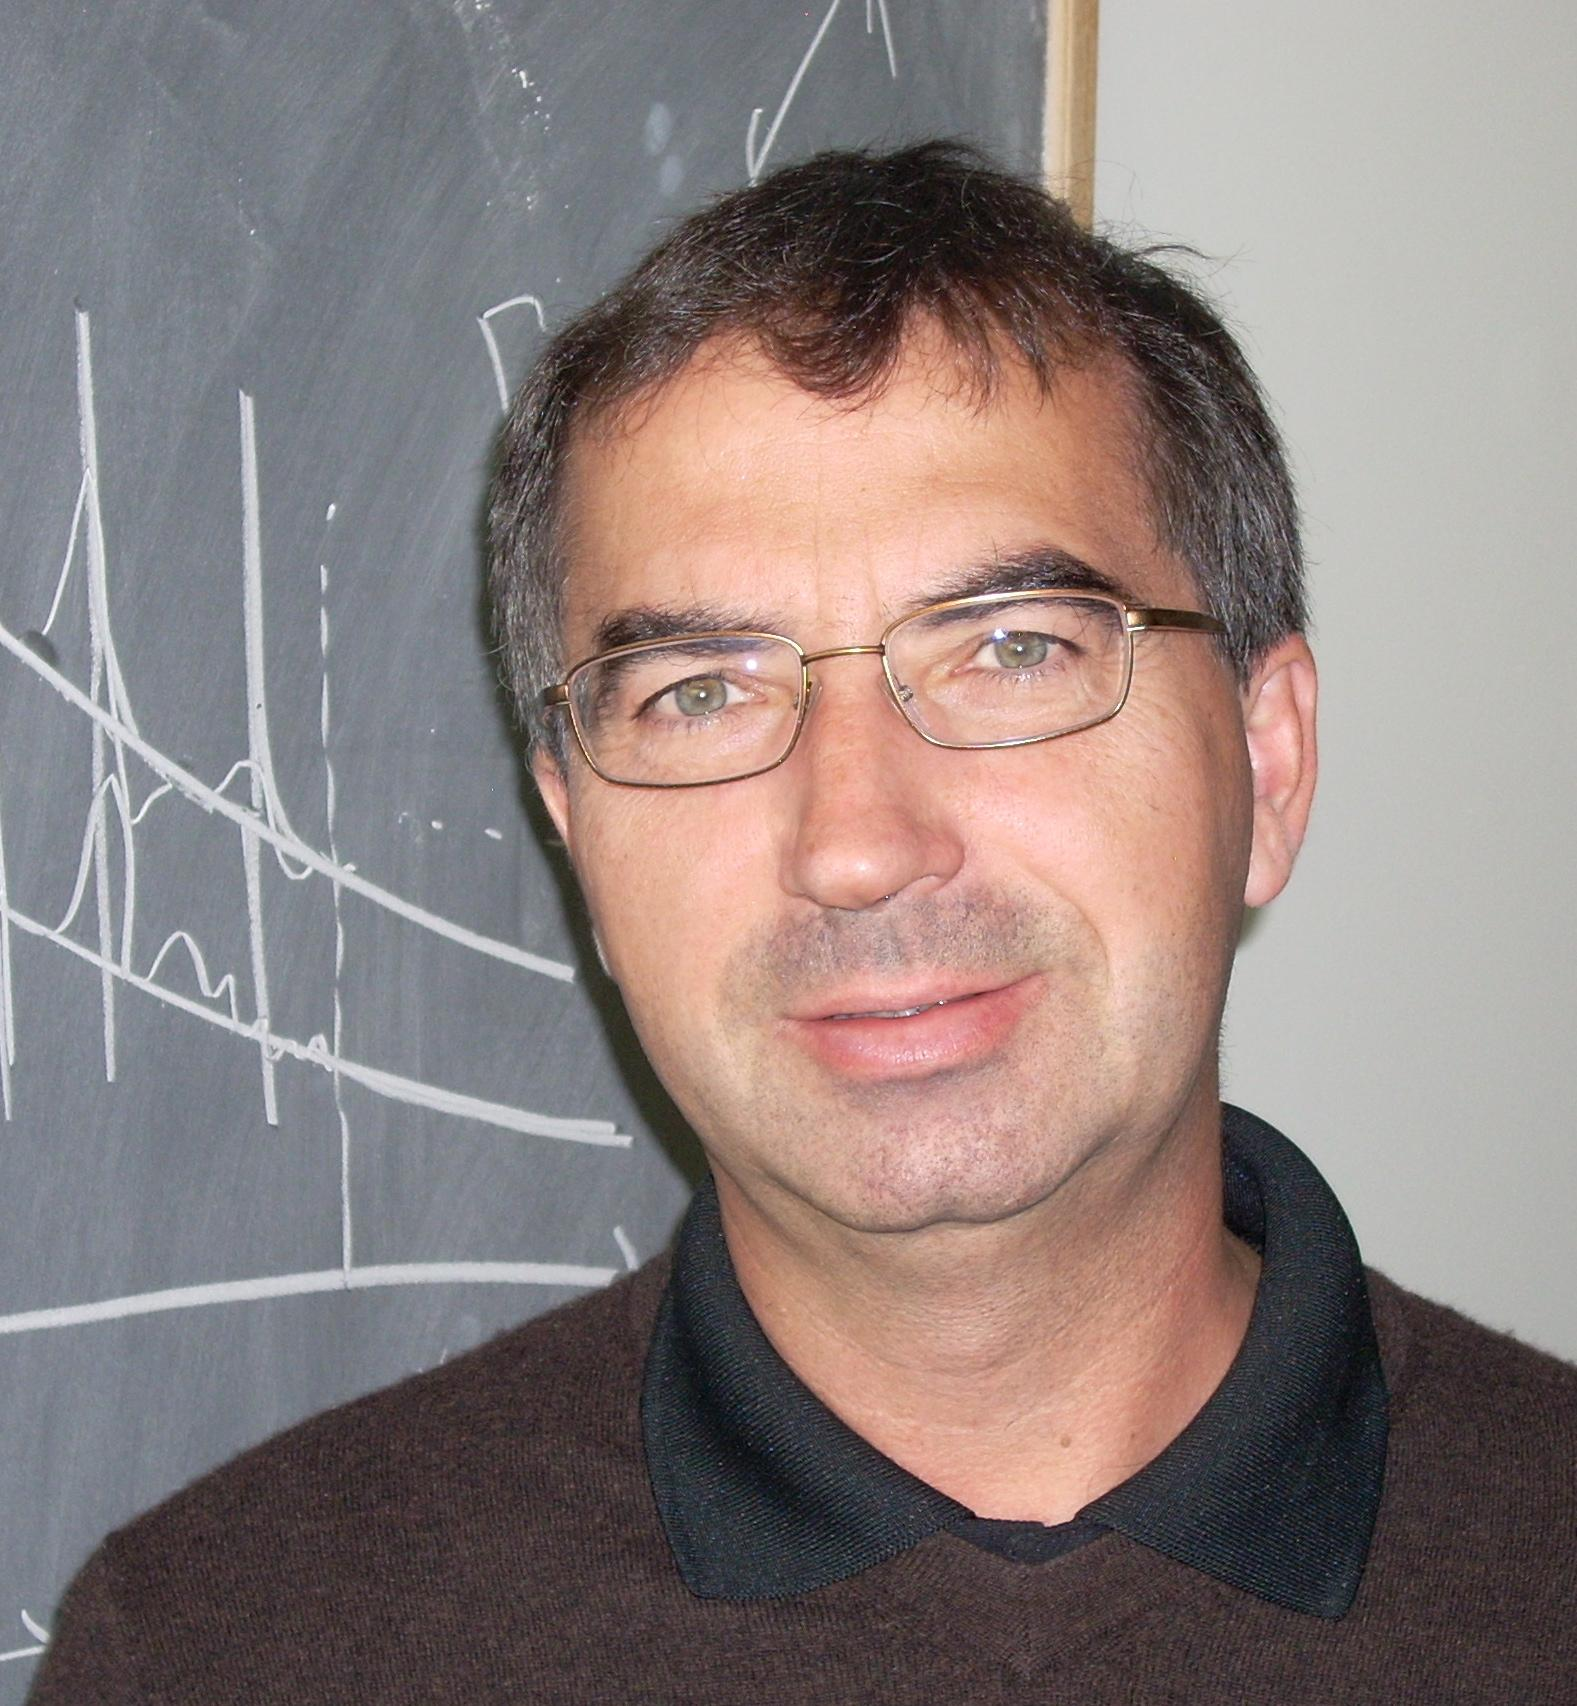
\includegraphics[width=3cm]{figures/petr.jpeg}
            \caption{Petr Navratil}
         \end{subfigure}
            \caption{(TRIUMF)}
         \end{figure}
      %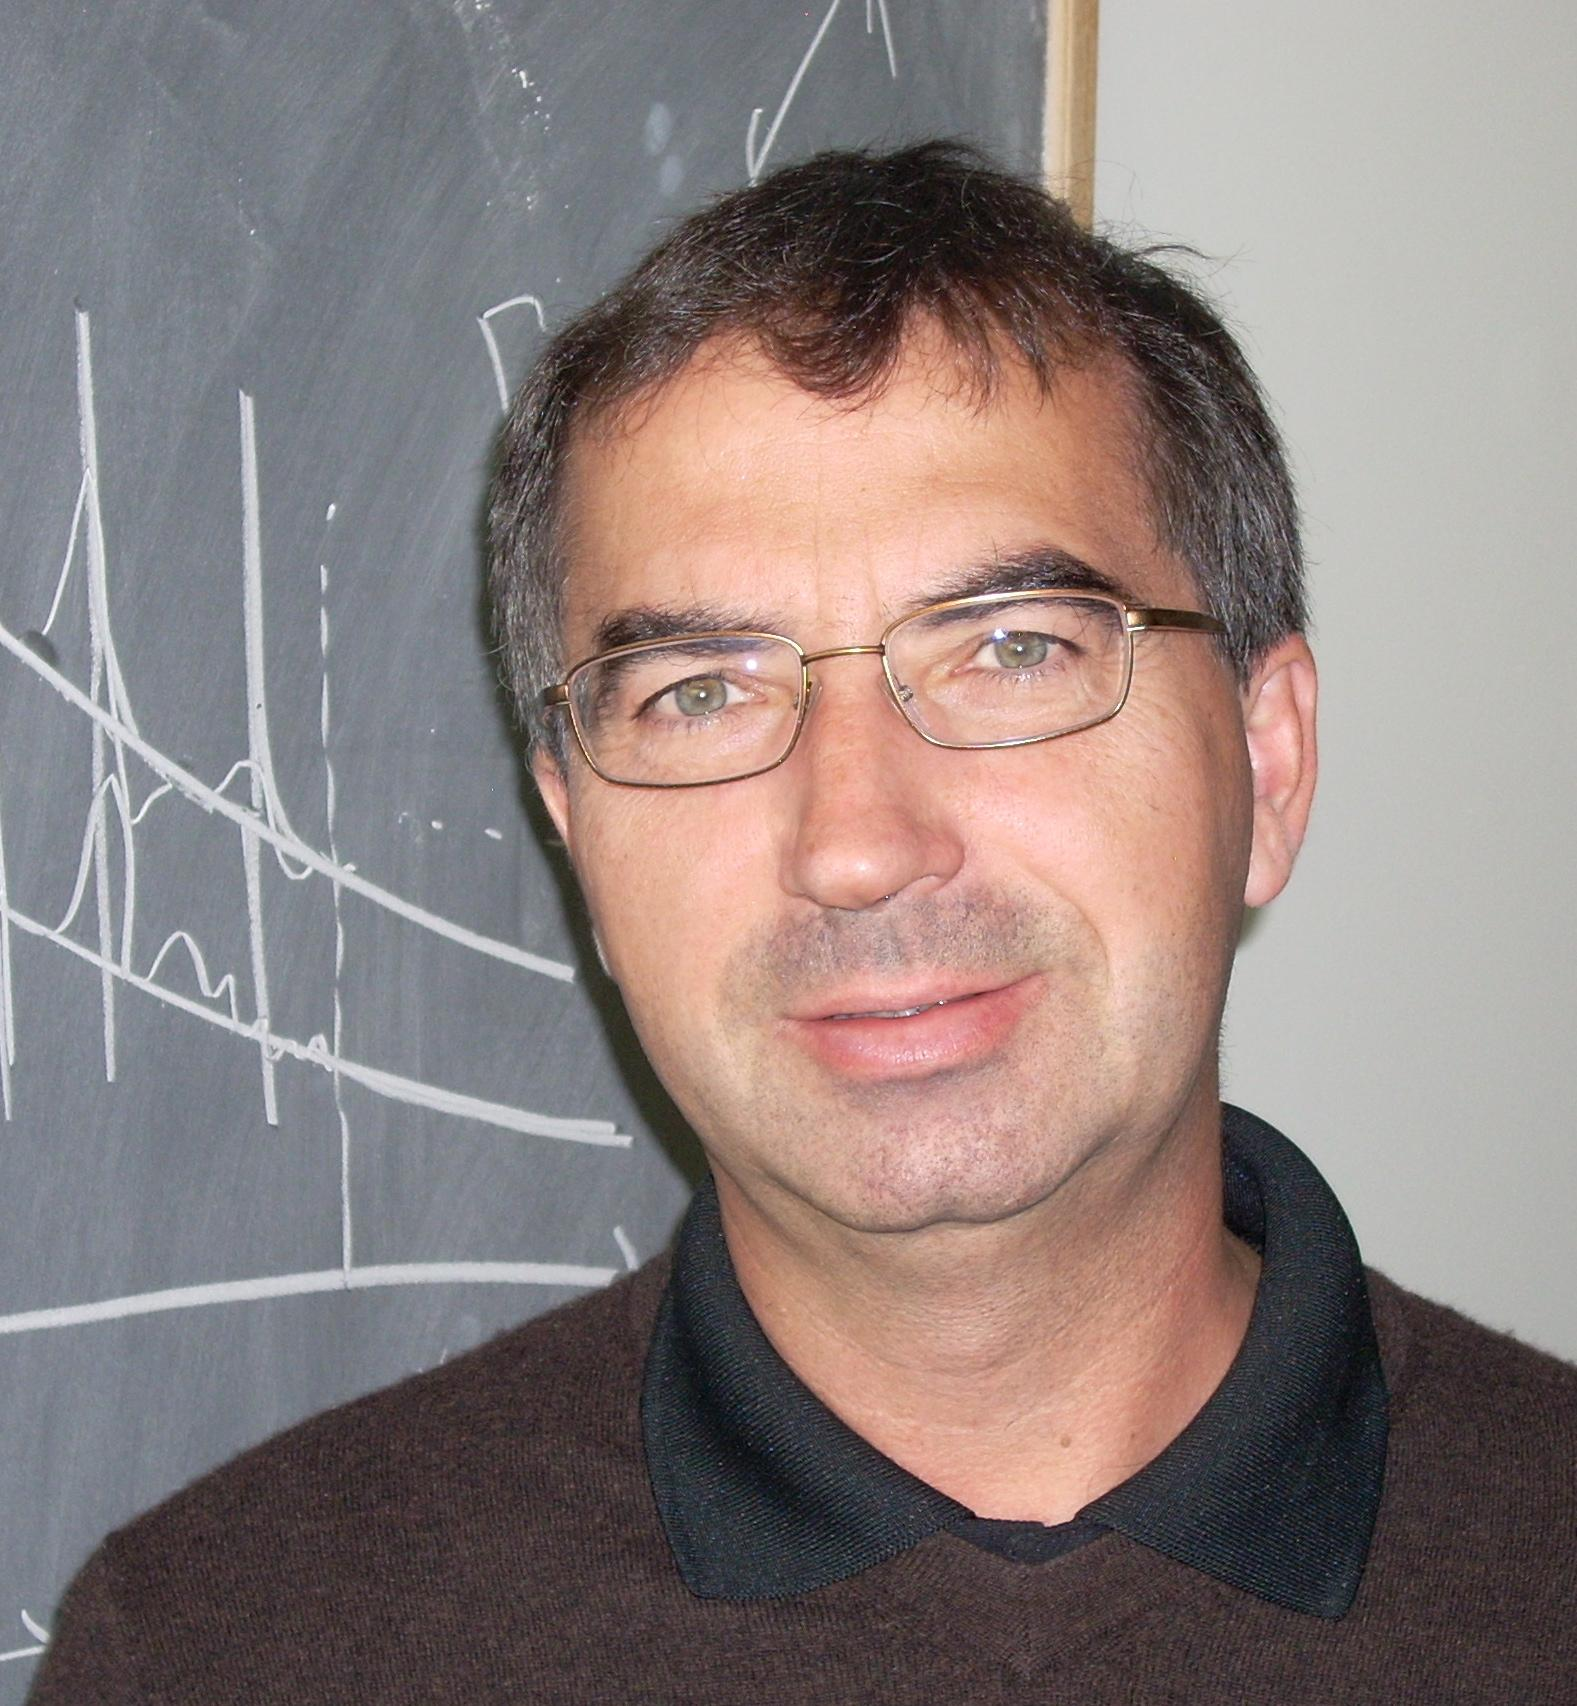
\includegraphics[scale=0.05]{figures/petr.jpeg}
         \end{center}
         \vspace{-0.5cm}
      \end{varblock}
   \end{textblock*}


\end{frame}

\end{document}
